% fig_overview — DeltaCycle system overview (TikZ + pgfplots, standalone)
\documentclass[border=2pt]{standalone}
\usepackage[T1]{fontenc}
\usepackage{lmodern}
\usepackage{xcolor}
\usepackage{pgfplots}
\pgfplotsset{compat=1.16}
\usetikzlibrary{arrows.meta,positioning,calc,fit}

\definecolor{ink}{RGB}{34,48,58}
\definecolor{teal}{RGB}{61,122,138}
\definecolor{sage}{RGB}{156,179,128}
\definecolor{blue}{RGB}{122,155,181}
\definecolor{coral}{RGB}{217,139,106}
\definecolor{sand}{RGB}{224,201,166}
\definecolor{boxbg}{RGB}{244,246,247}
\definecolor{edge}{RGB}{191,204,210}
\definecolor{titlebg}{RGB}{253,246,227}

\tikzset{
  panel/.style={draw=edge,line width=0.5pt,fill=boxbg,rounded corners=3pt},
  chip/.style={draw=edge,thin,fill=#1,rounded corners=2pt,
    font=\scriptsize,align=center,inner sep=2.5pt},
  photocard/.style={draw=edge,thin,inner sep=0pt},
}

\begin{document}
\begin{tikzpicture}
  \node[fill=titlebg,draw=edge,rounded corners=3pt,font=\bfseries\large,
        minimum width=15.6cm,minimum height=0.8cm] at (8,8.55)
        {DeltaCycle --- capacity-only battery monitoring loop};

  % ---- left: 6 scene photos ----
  \node[photocard] at (1.05,7.40)
    {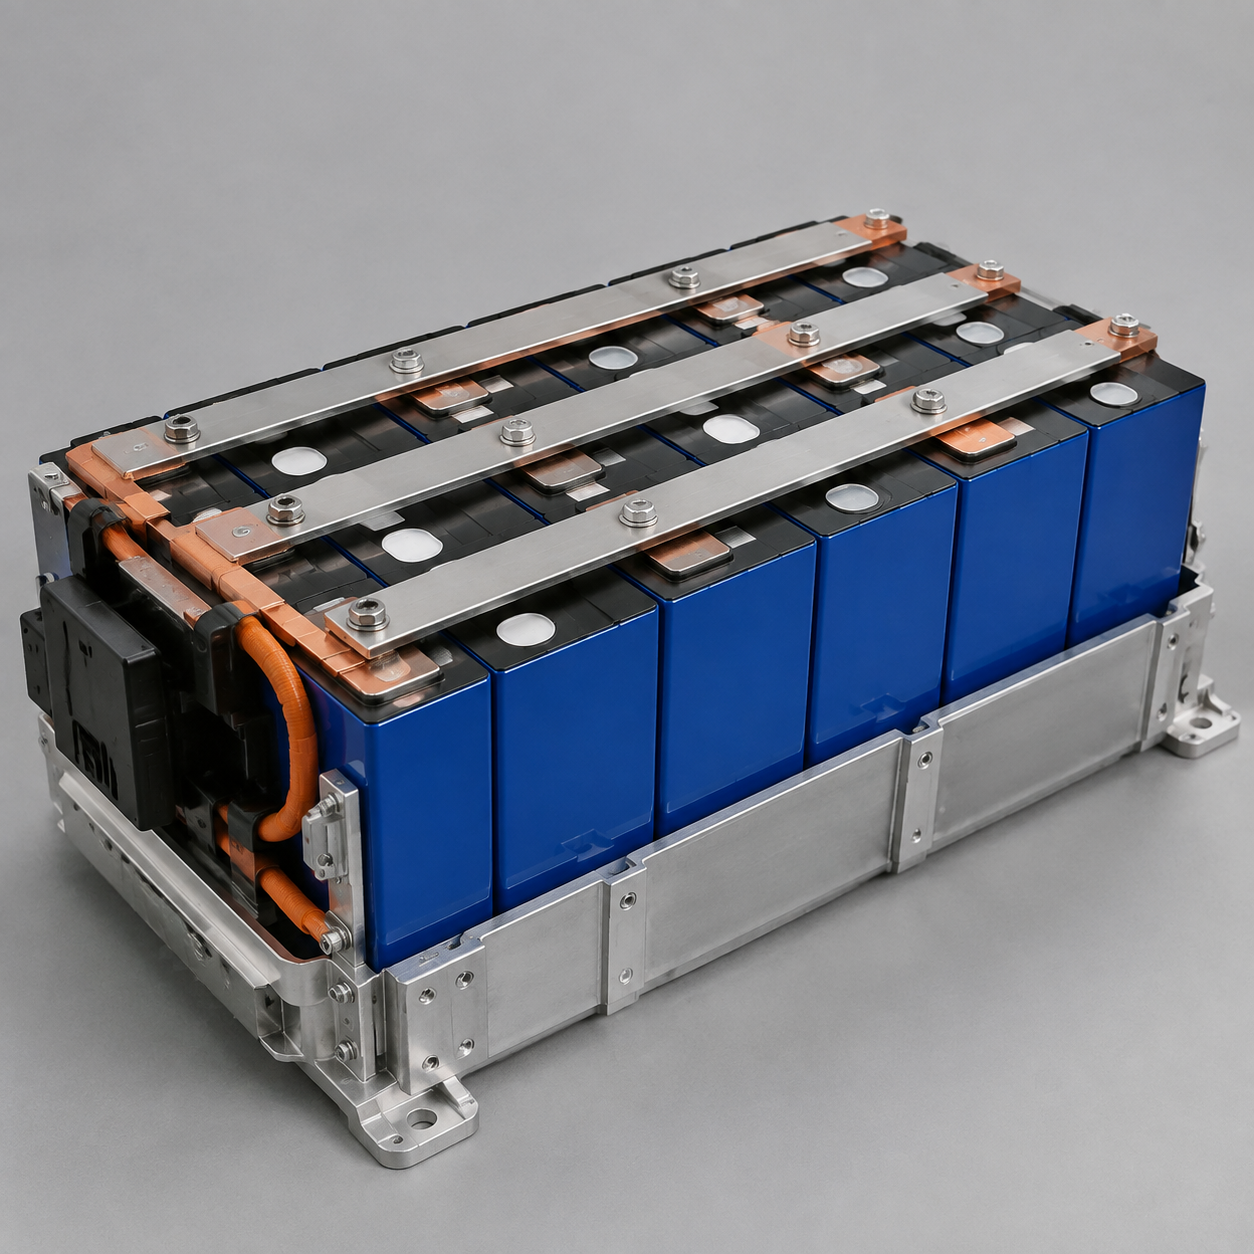
\includegraphics[width=1.18cm,height=1.18cm]{../photos/ev_pack.png}};
  \node[below=1pt,font=\tiny] at (1.05,6.78) {EV fleets};
  \node[photocard] at (2.55,7.40)
    {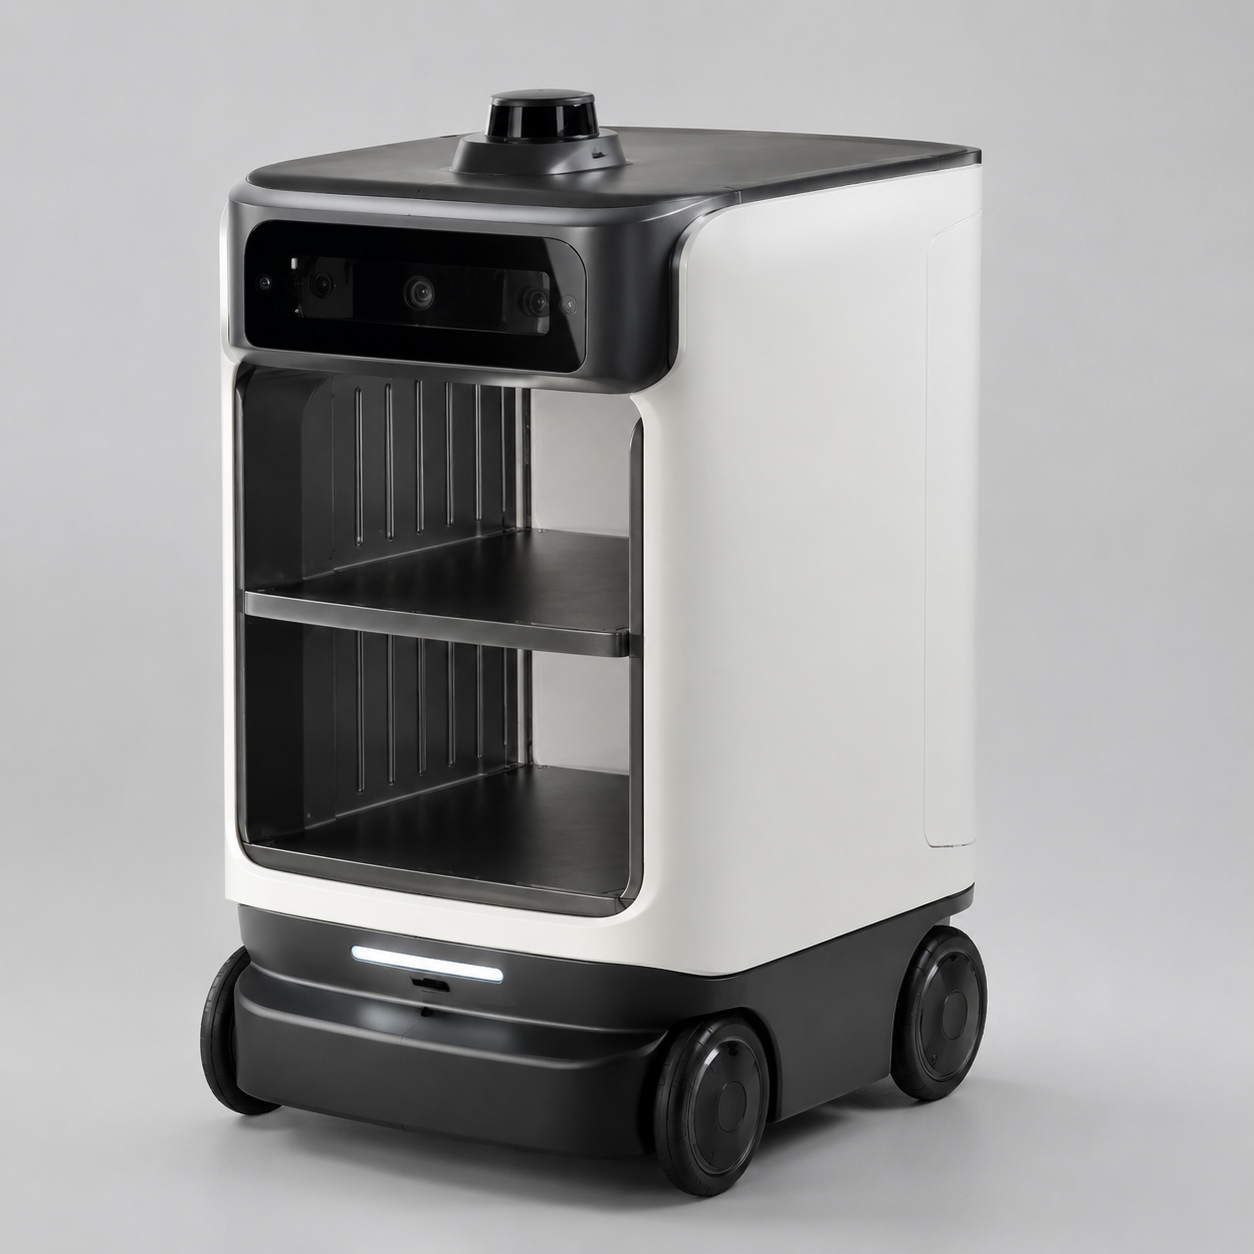
\includegraphics[width=1.18cm,height=1.18cm]{../photos/robot.png}};
  \node[below=1pt,font=\tiny] at (2.55,6.78) {Robot fleets};
  \node[photocard] at (4.05,7.40)
    {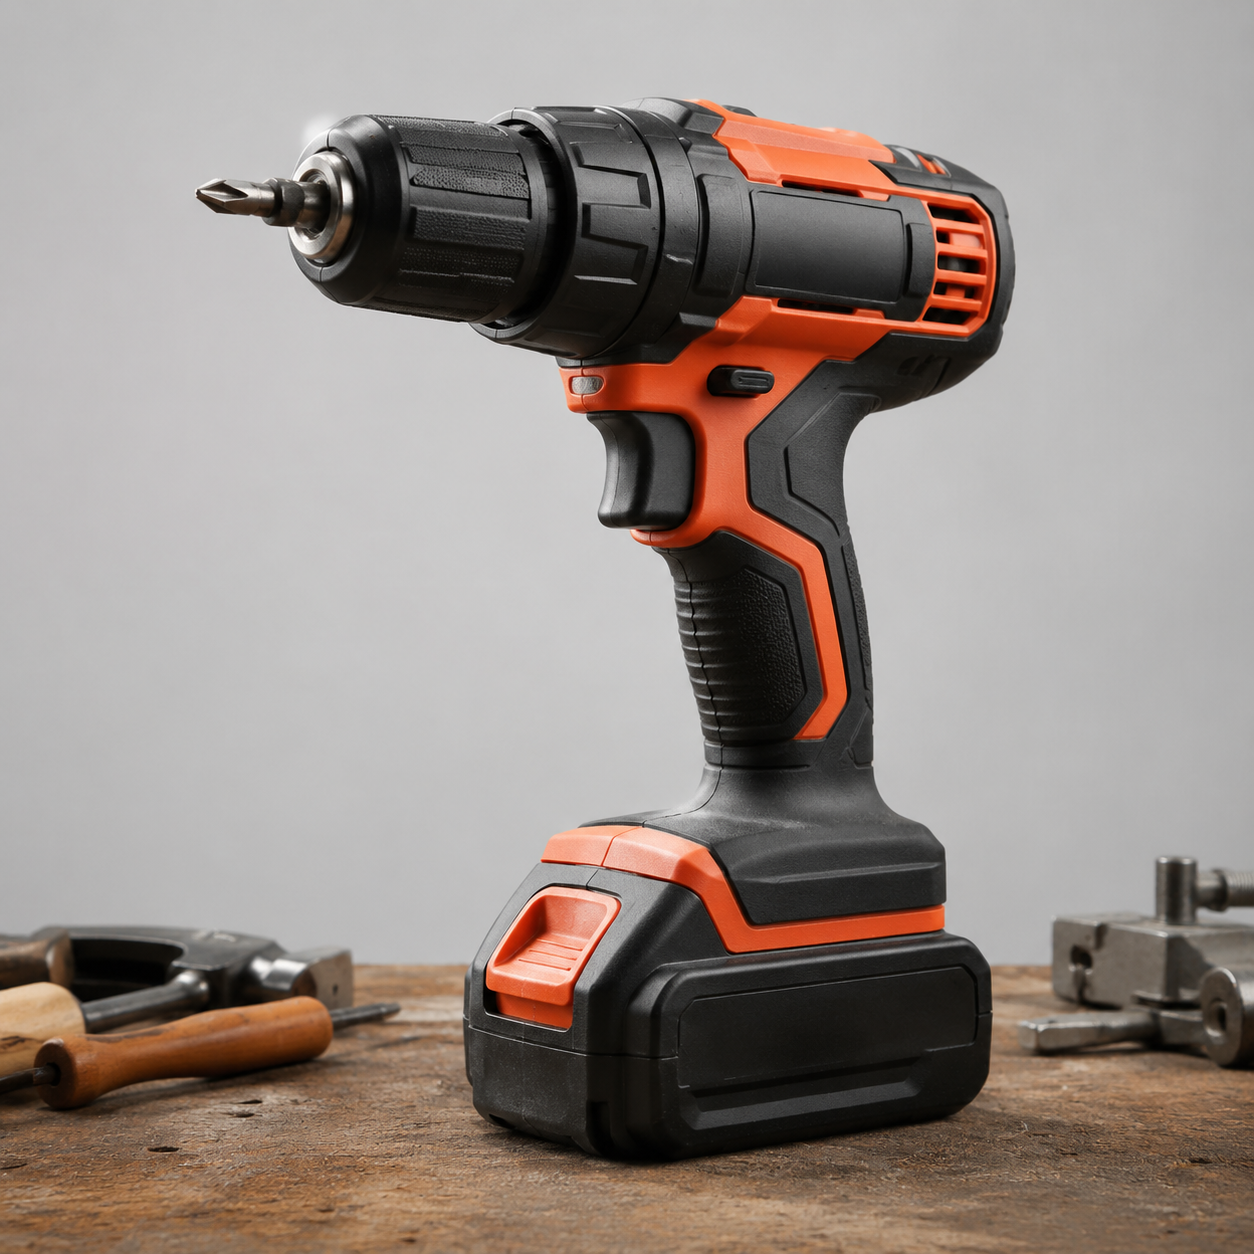
\includegraphics[width=1.18cm,height=1.18cm]{../photos/power_tool.png}};
  \node[below=1pt,font=\tiny] at (4.05,6.78) {Power tools};
  \node[photocard] at (1.05,5.45)
    {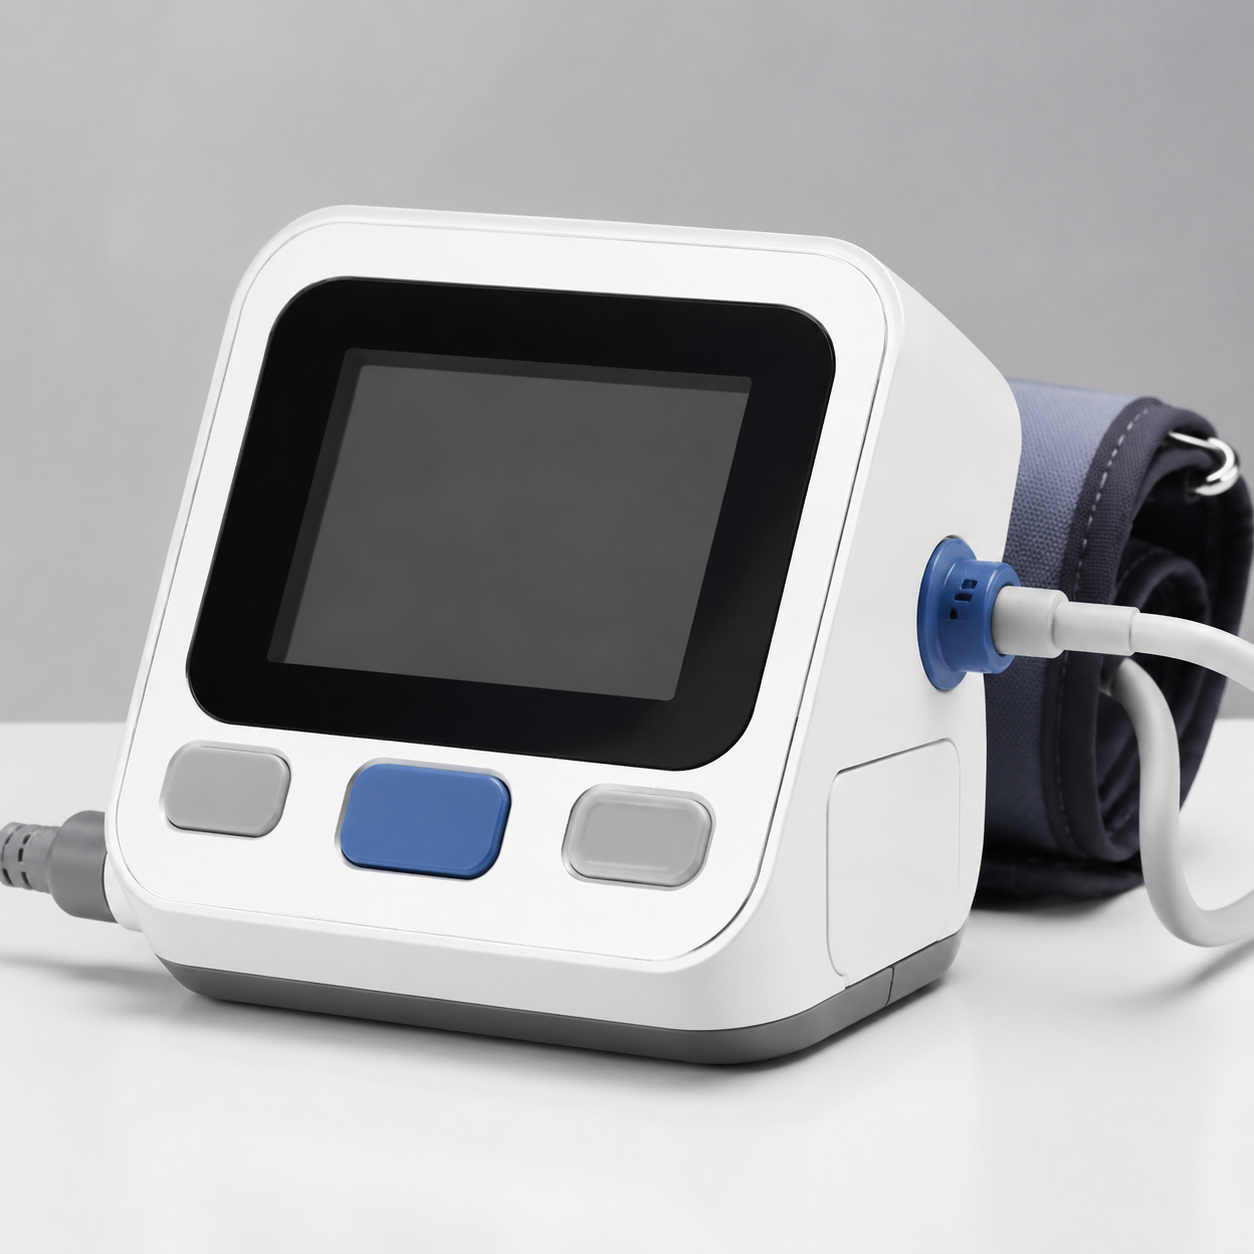
\includegraphics[width=1.18cm,height=1.18cm]{../photos/medical.png}};
  \node[below=1pt,font=\tiny] at (1.05,4.83) {Medical devices};
  \node[photocard] at (2.55,5.45)
    {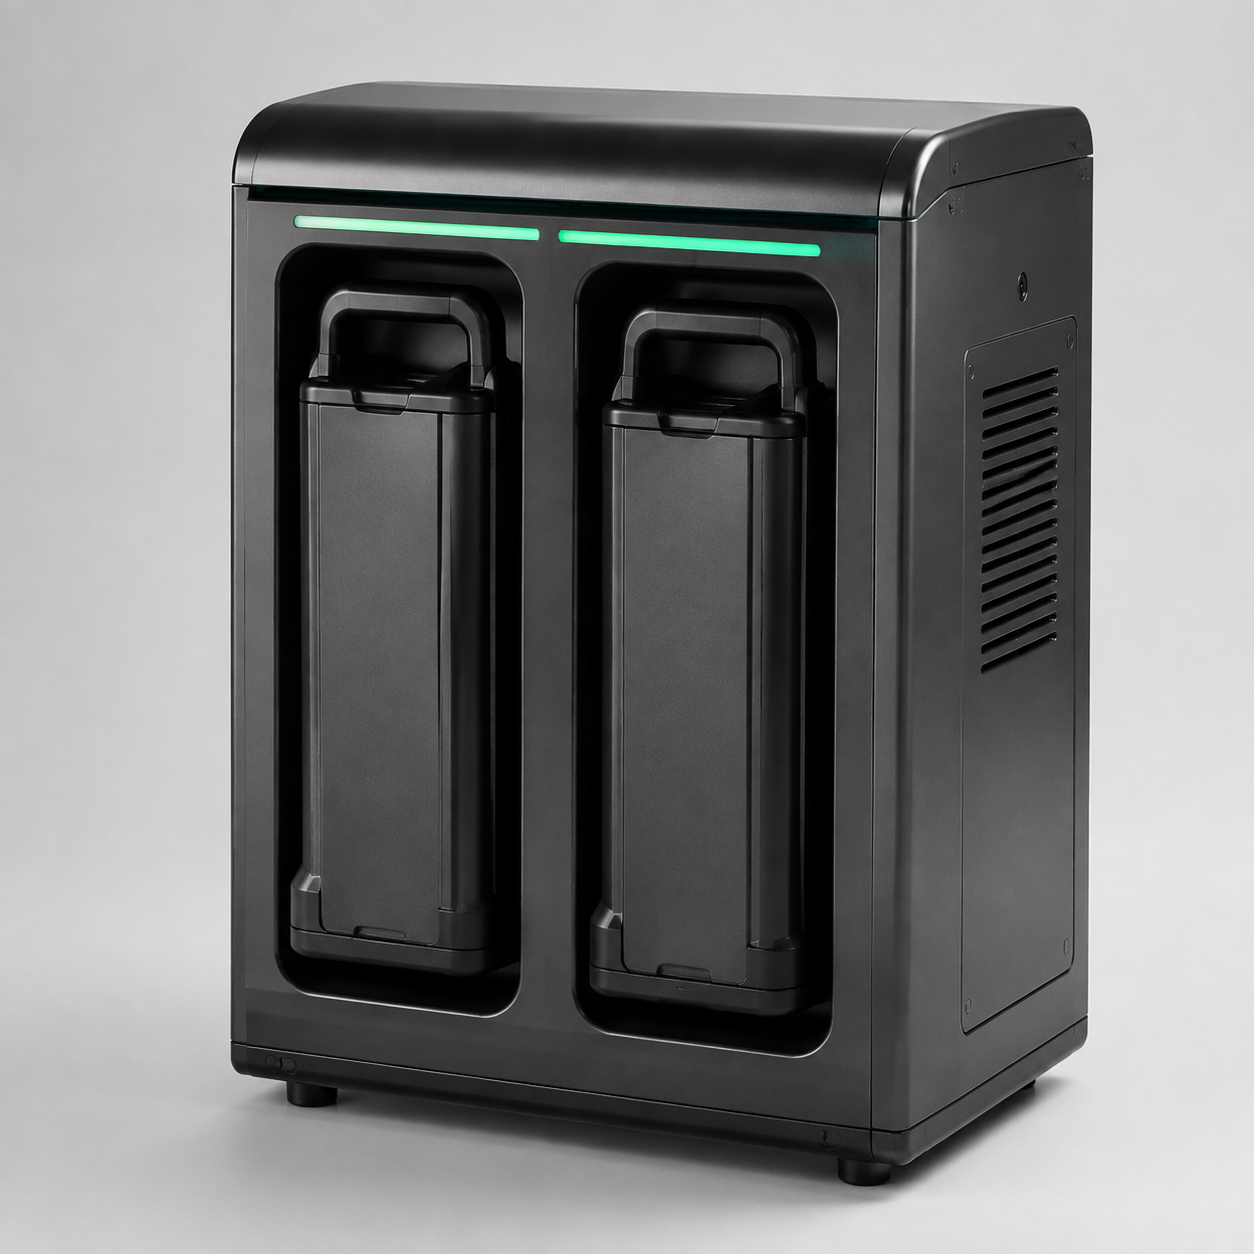
\includegraphics[width=1.18cm,height=1.18cm]{../photos/ebike.png}};
  \node[below=1pt,font=\tiny] at (2.55,4.83) {E-bike swap};
  \node[photocard] at (4.05,5.45)
    {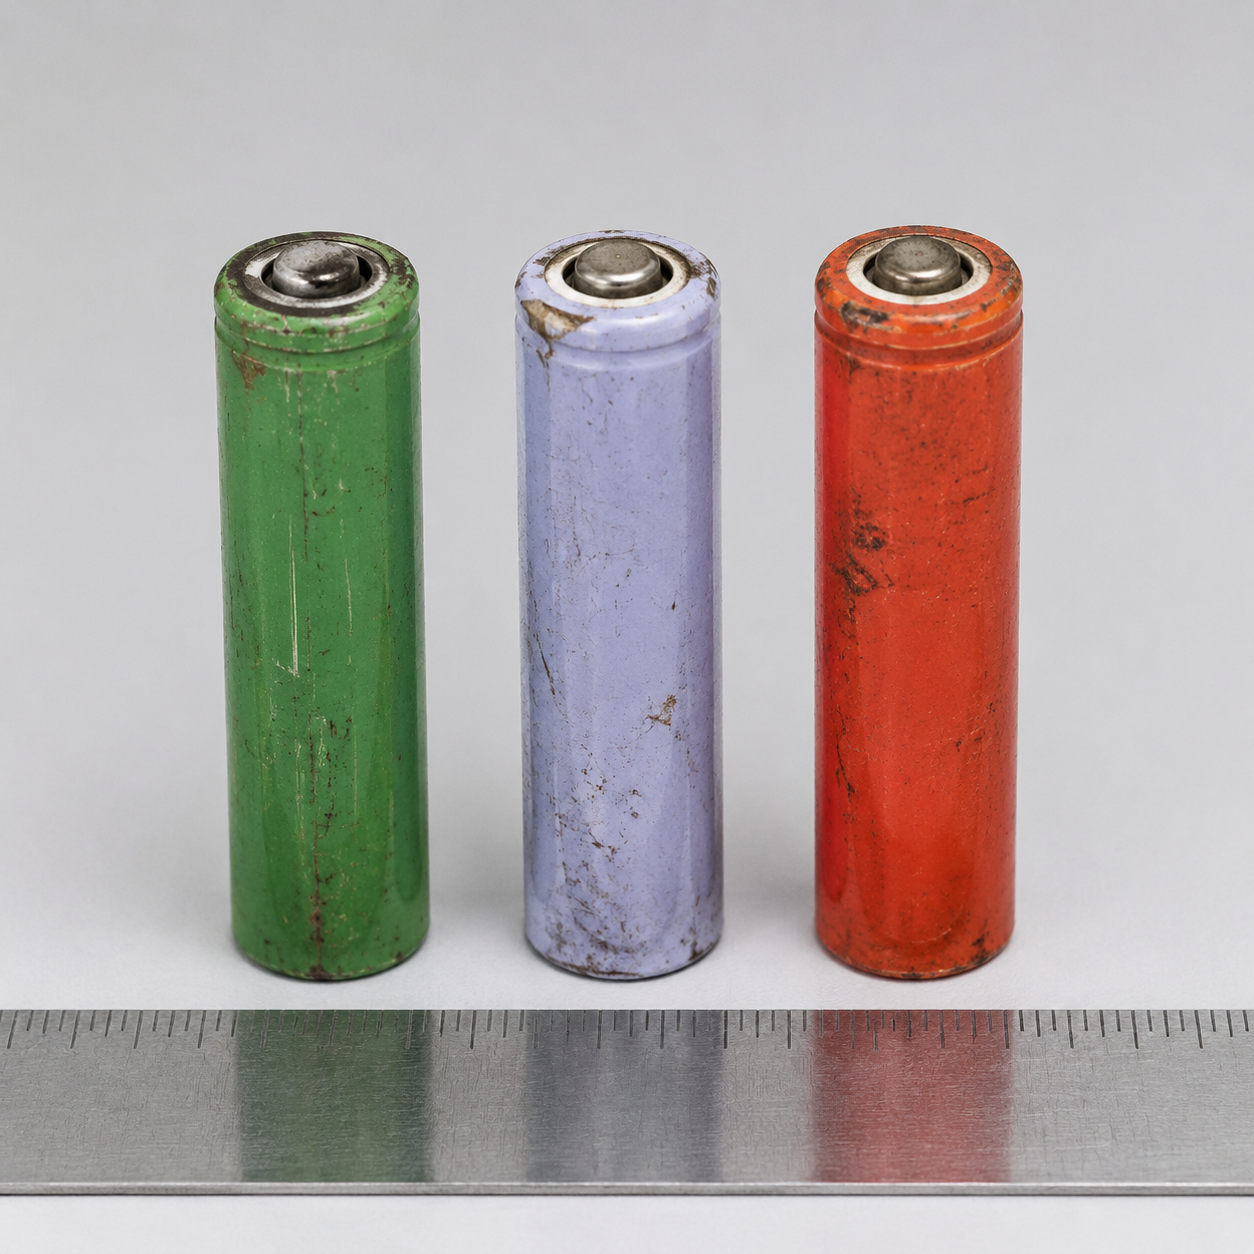
\includegraphics[width=1.18cm,height=1.18cm]{../photos/second_life.png}};
  \node[below=1pt,font=\tiny] at (4.05,4.83) {Second-life};

  % ---- right: 4 panels ----
  \draw[panel] (4.80,1.30) rectangle (7.42,6.60);
  \draw[panel] (7.80,1.30) rectangle (10.42,6.60);
  \draw[panel] (10.80,1.30) rectangle (13.42,6.60);
  \draw[panel] (13.80,1.30) rectangle (16.42,6.60);
  \node[fill=teal,rounded corners=2pt,minimum width=2.40cm,minimum height=0.5cm,
        text=white,font=\bfseries\footnotesize,align=center]
    at (6.11,6.32) {A  Accurate monitoring};
  \node[fill=sage,rounded corners=2pt,minimum width=2.40cm,minimum height=0.5cm,
        text=white,font=\bfseries\footnotesize,align=center]
    at (9.11,6.32) {B  Physics foresight};
  \node[fill=blue,rounded corners=2pt,minimum width=2.40cm,minimum height=0.5cm,
        text=white,font=\bfseries\footnotesize,align=center]
    at (12.11,6.32) {C  Trustworthy decisions};
  \node[fill=coral,rounded corners=2pt,minimum width=2.40cm,minimum height=0.5cm,
        text=white,font=\bfseries\footnotesize,align=center]
    at (15.11,6.32) {D  Edge deployment};

  % A
  \begin{scope}[shift={(4.95,2.85)}]
  \begin{axis}[width=2.32cm,height=2.55cm,anchor=south west,
      axis lines=left,line width=0.4pt,label style={font=\tiny},
      tick label style={font=\tiny},ylabel={norm.\ cap.},xlabel={cycle},
      ymin=0,ymax=1.05,xtick={0,400,800},ytick={0,0.5,1.0}]
    \addplot[teal,line width=0.7pt,mark=none]
      table[x index=0,y index=1]{../data/capacity.dat};
  \end{axis}
  \end{scope}
  \node[chip=boxbg,minimum width=2.30cm] at (6.11,1.92)
        {SOTA trajectory accuracy\\regeneration tracked};

  % B
  \begin{scope}[shift={(7.95,2.85)}]
  \begin{axis}[width=2.32cm,height=2.55cm,anchor=south west,
      axis lines=left,line width=0.4pt,label style={font=\tiny},
      tick label style={font=\tiny},ylabel={norm.\ cap.},xlabel={cycle},
      legend style={font=\tiny,draw=none,cells={anchor=west},
                    at={(0.02,0.98)},anchor=north west},
      ymin=0,ymax=1.05,xtick={800,840,880}]
    \addplot[ink,line width=0.6pt,mark=none]
      table[x index=0,y index=1]{../data/ext.dat}; \addlegendentry{truth}
    \addplot[blue,dashed,line width=0.6pt,mark=none]
      table[x index=0,y index=2]{../data/ext.dat}; \addlegendentry{free head}
    \addplot[coral,line width=0.8pt,mark=none]
      table[x index=0,y index=3]{../data/ext.dat}; \addlegendentry{rate head}
  \end{axis}
  \end{scope}
  \node[font=\tiny\color{coral},anchor=south east] at (10.25,2.90)
        {extR$^2$ 0.775};
  \node[chip=boxbg,minimum width=2.30cm] at (9.11,1.92)
        {unseen-tail extrapolation};

  % C
  \begin{scope}[shift={(10.95,2.85)}]
  \begin{axis}[width=2.32cm,height=2.55cm,anchor=south west,
      axis lines=left,line width=0.4pt,label style={font=\tiny},
      tick label style={font=\tiny},ylabel={norm.\ cap.},xlabel={cycle},
      ymin=0,ymax=1.05,xtick={0,400,800},ytick={0,0.5,1.0}]
    \addplot[teal,line width=0.7pt,mark=none]
      table[x index=0,y index=1]{../data/capacity.dat};
    \addplot[blue!30,line width=0pt,fill opacity=0.35]
      {0.55 - 0.25*x/880 + 0.03*sin(deg(x/880*6))} \closedcycle;
  \end{axis}
  \end{scope}
  \node[font=\tiny,anchor=south east] at (13.25,2.90) {coverage 0.933};
  \node[chip=boxbg,minimum width=2.30cm] at (12.11,1.92)
        {risk-aware scheduling};

  % D
  \node[photocard] at (15.11,4.30)
    {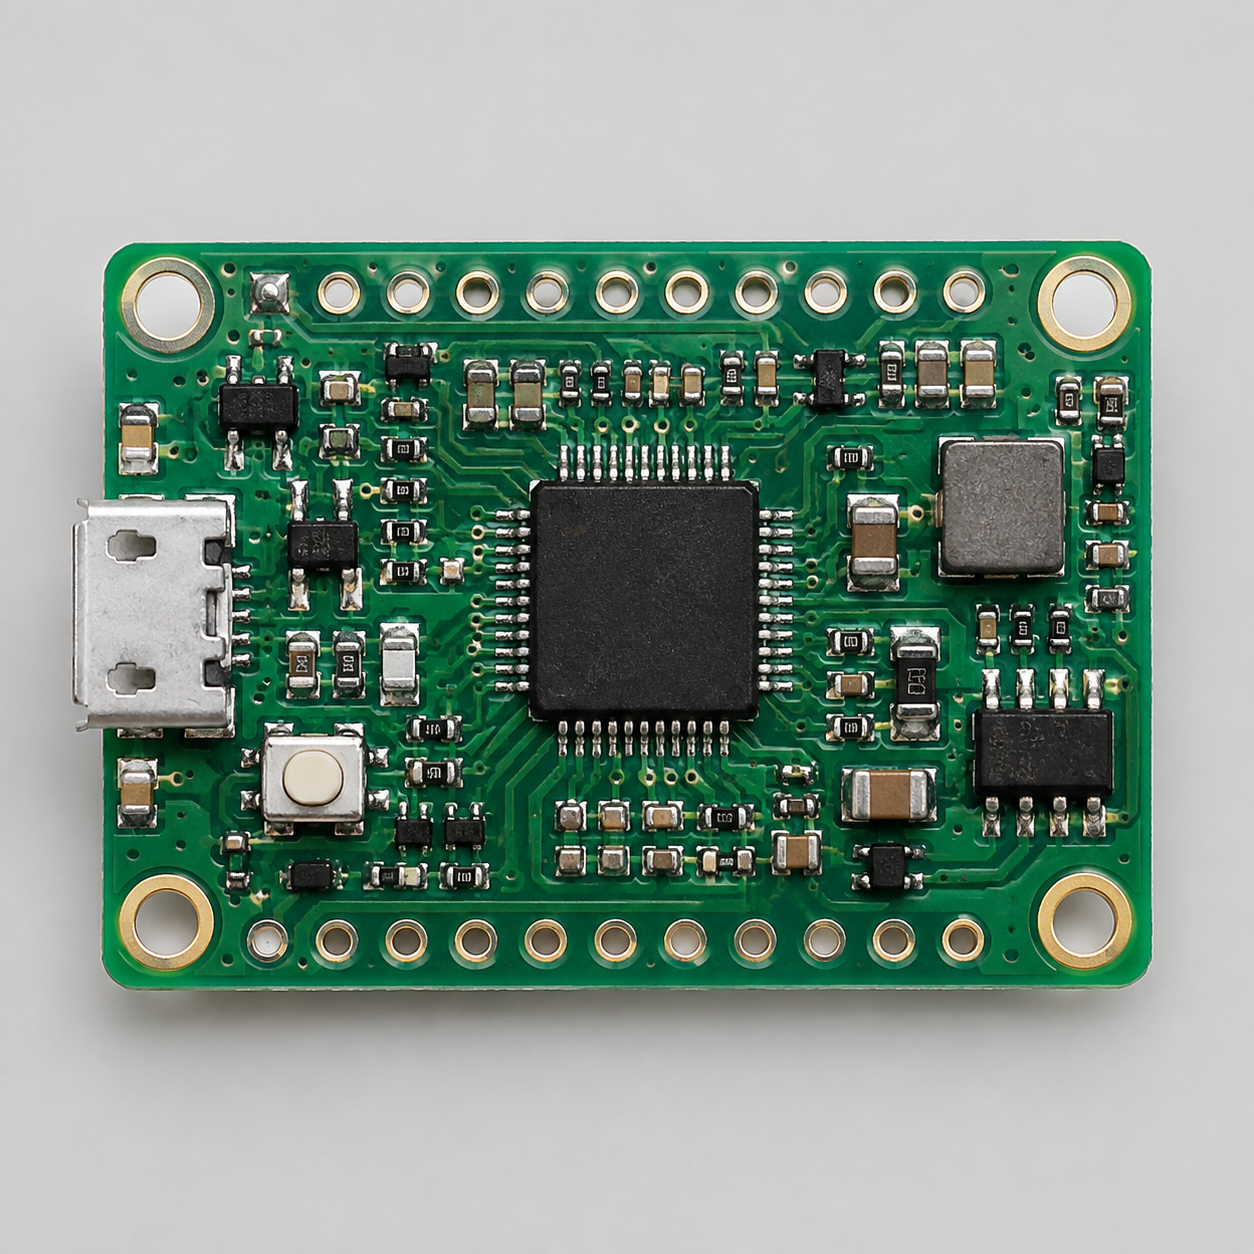
\includegraphics[width=1.65cm,height=1.65cm]{../photos/mcu_board.png}};
  \node[font=\scriptsize,color=blue!70!black] at (15.11,3.35)
        {STM32-class MCU};
  \node[chip=sand,minimum width=2.30cm] at (15.11,2.70) {fixed 8 KB state};
  \node[chip=sand,minimum width=2.30cm] at (15.11,2.10) {INT8 340 KB};
  \node[chip=sand,minimum width=2.30cm] at (15.11,1.50) {no cloud};

  \node[fill=boxbg,draw=edge,rounded corners=3pt,font=\normalsize,
        minimum width=11.6cm,minimum height=0.85cm] at (10.61,0.45)
        {MAE 0.0049 $\vert$ R$^2$ 0.9945 $\vert$ AE 1.2 cycle $\vert$
         5 datasets, 12 SPs, 10 seeds};
\end{tikzpicture}
\end{document}
